\section{Introduction}
By now we all want to configure the cisco devices such as routers and switches. Cisco devices do include GUIs - which means graphical user interface - but in the real world, everybody just uses the command line interface (CLI) because it is much quicker than using the GUIs. The OS used in enterprise grid cisco devices is IOS, in this section we'll learn how to connect to the devices and the use of the command line. A disclaimer is that the IOS operating system is not the only one, there are others.


%----------------------------------------------------------------------------------------
\section{Cisco operating systems}
Cisco history is not going to be examined on the CCNA exam. Neil includes this just because of context. Cisco IOS and the other OS's work basically the same way in terms of management and administrative point of view, the operating systems don't differ that much in terms of how you use it, maybe on how they are actually implemented but not really on how you use it. By learning cisco IOS you are really learning all of the others at once.

\subsection{A short history of cisco operating systems}
\begin{itemize}
    \item Most people think of cisco as primarily a routing and switching company, but they actually started out with just routers in 1984. 
    \item IOS was the original operating system that they used on routers - the same OS they use today (with some optimizations).
    \item IOS is the operating system that has been used on cisco routers since their inception.
    \item Cisco Catalyst switches evolved from the acquisition of Crescendo company in 1993 - cisco bought the company Crescendo- and started manufacturing switches of which the first one was Catalyst. 
    \item The original cisco switch operating system was CatOS which has not been deprecated.
    \item Cisco firewalls evolved from the acquisition of the company Network Translation's PIX firewall that uses the Finesse operating system in 1995.
    \item Cisco switches and firewalls (now the ASA firewall) were ported over the IOS operating system over the following years.
    \item Cisco standardized on IOS for all the network infrastructure devices.
\end{itemize}
There are some other operating systems in some newer router and switch platform. IOS runs on the majority of routers and switches. Some of these other operating systems are:
\begin{itemize}
    \item The Cisco Nexus and MDS data center switch product lines run on NX-OS.
    \item The IOS-XR operating system runs on the service provider NCS, CRS, ASR9000, and XR12000 series routers (these are the higher end routers).
    \item IOS-XE runs on the ASR1000 series service provider routers (1K service providers).
    \item The command line interfaces for teh other operating systems are nearly identical to IOS.
\end{itemize}
At first all of these names might seem intimidating but fear not, all of the OS's run nearly identical commands, if you can use one, you can practically use them all. There are different OS's because they are implemented with different functionality, for example, IOS has a monolithic kernel - which means that if one process crashes it crashes the entire router - they are all different under the hood. Other OS's have different kernels to permit that if one crashes the other processes in the router are not affected, only that process is crashed. This is does not mean that IOS is bad or unreliable, it simply means that it works differently given different situations.


%----------------------------------------------------------------------------------------
\section{Connecting to a cisco device over the network}
\begin{itemize}
    \item The lab exercises in this course use Cisco Packet Tracer simulation software on your PC.
    \item This lecture shows how to connect to a real router or switch over the network with Putty - which a software to connect to routers - you are not going to use Putty in the labs because everything is done in the Packet Tracer simulation software.
    \item You do not need to install or use Putty to do the course lab exercises.
\end{itemize}

\subsection{Connecting over the network}
In you day-to-day as a network engineer you are typically not going to be connecting stuff, instead you are going to be in your desk 'working remotely', you are going to be connecting to that device over the network. So the following example: Let's say that you are in a London office and want to establish a connection in the NY office. What you are going to do is use software on your PC, connect to the router over the network in NY, get to the command line of device you want to work on, and get on with your job.
\begin{figure}[H]
    \centering
    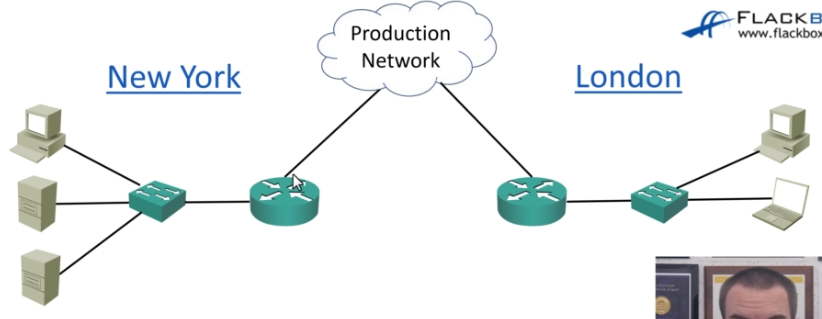
\includegraphics[width=\width\textwidth]{./Figs/2021-10-12-14-23-26.png}
% 	\caption{}
\end{figure}
\begin{itemize}
    \item To get to the CLI for day-to-day management of a Cisco device you will use Secure Shell (SSH) to connect to it's management IP addresses over the network.
    \item There is also another protocol called Telnet which is also supported but not recommended because it is insecure. Commands in Telnet are un-encrypted, so anybody listening in to your traffic can get ahold of data, including username and password. Telnet is never used in a real setting for the potential vulnerabilities. In reality SSH is always used, Telnet is almost always used only on a lab environment to learn.
    \item In enterprise networks, secure login will typically be enforced through intergration with a centralized AAA (Authentication, Authorization, and Accounting) server.
        \begin{itemize}
            \item Basically the AAA server is a solution to many people loggin in. In a network, you can probably have many devices with username and passwords that must be verified to be granted access to network actions. We don't want each device to have the username and passwords of all the others so we centralize that into one server that stores all the user name and passwords that has access to the central database of usernames and passwords.
        \end{itemize}
\end{itemize}

\subsection{Installing Putty}
Installing Putty is basically just searching on Google and accepting all the defaults once the executable has been downloaded. When you launch the window you will be faced with a window like this: 
\begin{figure}[H]
    \centering
    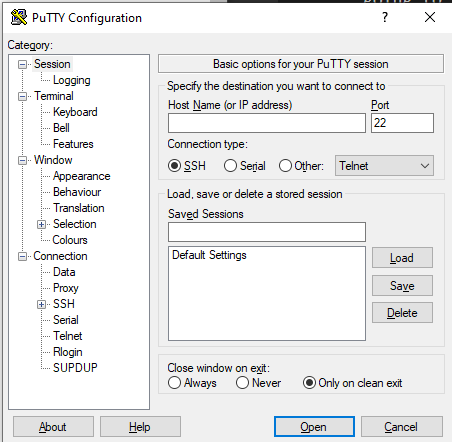
\includegraphics[width=\width\textwidth]{./Figs/2021-10-12-14-19-06.png}
% 	\caption{}
\end{figure}
The host name refers to the host that I am intending to connect to, it takes as an input an IP address. Then you log in through the command line, and type your password. This is how you connect to a cisco device, very simple using Putty.

\subsection{Out of band management}
To continue the example in which we were connecting in London to the NY office, we are essentially using the production network. But most large companies use a separate management network, this is done as a backup path in case the production network is down, it is also more secure to have a separate dedicated path. The production network is the in band network, which means you are using the same cables that your normal users (your staff) are using to connect to other devices. If you connect to the NY office through the management network you are using and out of band network, which means you are not using the same network as the normal staff. Trivial difference but important distinction.
\begin{figure}[H]
    \centering
    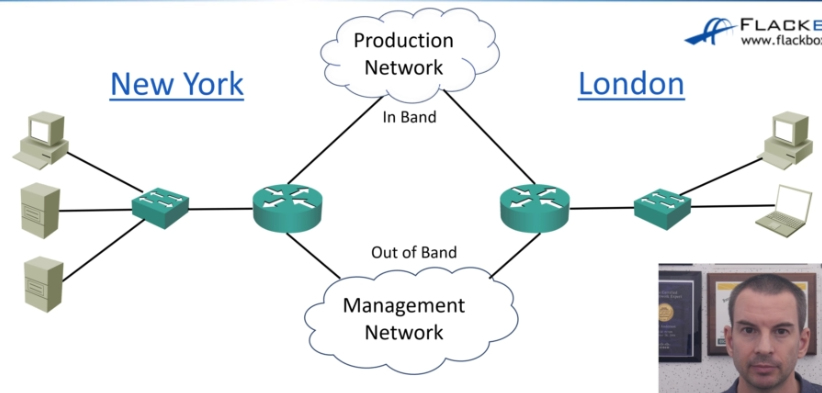
\includegraphics[width=\width\textwidth]{./Figs/2021-10-12-14-28-22.png}
% 	\caption{}
\end{figure}


%----------------------------------------------------------------------------------------
\section{Making the initial connection to a cisco device}
\begin{itemize}
    \item Cisco devices do not usually have a default IP address, so we need to set one up before we can connect to it over the network, but how do we connect to the device in the first place if we don't have an IP? 
    \item We need a way to connect to the device to do the initial configuration including adding IP addresses. This is where the console connection comes in. With a console connection we can connect to the device at a lower level below IP to get to the initial command line to do the initial configuration including adding an IP and finally be able to connect to it over the network.
\end{itemize}

For this initial configuration, we need a Console Cable (DB9 to RJ45) in order to connect to the router via a wire and send the configurations. Simply connect the cable to the console port on the router or switch and use the cable - which usually comes with your device.
\begin{figure}[H]
    \centering
    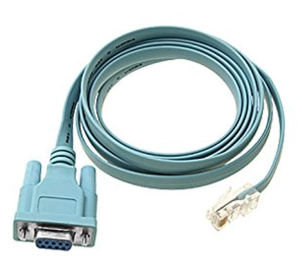
\includegraphics[width=0.4\textwidth]{./Figs/2021-10-14-22-28-42.png}
	\caption{Console Cable DB9 to RJ45}
\end{figure}

The console cable has two ends, one is the DB9 which is the thicker end, it is called that because it has 9 pins need to be connected to that end. 
\begin{figure}[H]
    \centering
    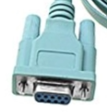
\includegraphics[width=0.4\textwidth]{./Figs/2021-10-14-22-29-57.png}
	\caption{DB9 end}
\end{figure}
The other end is very similar to an ethernet cable. However, THIS IS NOT AN ETHERNET CABLE. It is a RJ45, it is not using ethernet and it doesn't require IP addresses, this only grants you low level access to the command line. 
\begin{figure}[H]
    \centering
    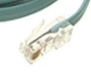
\includegraphics[width=0.4\textwidth]{./Figs/2021-10-14-22-31-28.png}
	\caption{RJ45}
\end{figure}
When you connect to make the initial configurations to the router using the console cable, the RJ45 - the one that looks like an ethernet connection but is not - end of the cable is the one that is going to be connected to the switch. The other end - the serial connector - plugs in to the computer. This is a problem for computers that don't include the DB9 connector, for this you can buy an adaptor from DB9 to USB.
\begin{figure}[H]
    \centering
    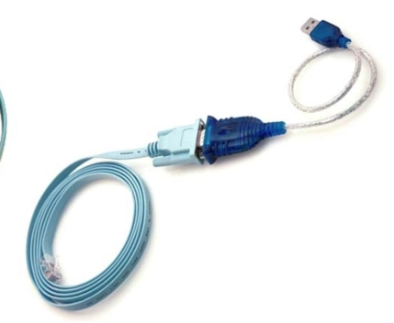
\includegraphics[width=0.4\textwidth]{./Figs/2021-10-14-22-33-54.png}
% 	\caption{}
\end{figure}

\subsection{Newer console cables}
With newer cisco devices the cable included comes already with a USB end for the computer since most computers don't come with DB9 cable support. So the newer console cables come with some modifications, not only the USB end for the computer but they actually removed the RJ45 ethernet looking but not ethernet end to be instead a microusb end.
\begin{figure}[H]
    \centering
    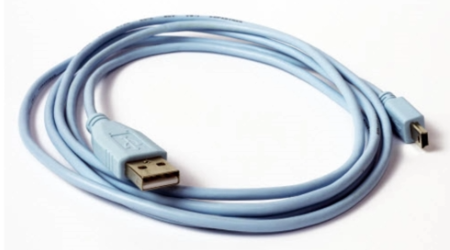
\includegraphics[width=0.4\textwidth]{./Figs/2021-10-14-22-37-53.png}
	\caption{USB to microusb}
\end{figure}

\subsection{Connecting via console cable to a real router}
First identify the console port on the router and connect the appropriate end (microusb or RJ45) to the router, the other end to your computer (USB or DB9). Launch putty and click that the connection type is going to be 'Serial'. Now you are going to have to specify your COM port correctly, if you don't know which one it is follow the following steps (windows):
\begin{itemize}
    \item Make sure that you have installed the driver software for the console cable in order for the COM port to be enabled.
    \item Open device manager and look in 'Ports (COM & LTP)'. 
        \begin{figure}[H]
            \centering
            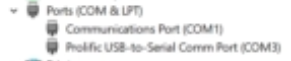
\includegraphics[width=0.4\textwidth]{./Figs/2021-10-14-22-44-59.png}
        % 	\caption{}
        \end{figure}
    
    \item In this case it is COM3, change in putty the COM<number> port specified in the device manager.
\end{itemize}
Then you need to select the speed, specified in the 'Serial' tab, and set flow control to None.
\begin{figure}[H]
    \centering
    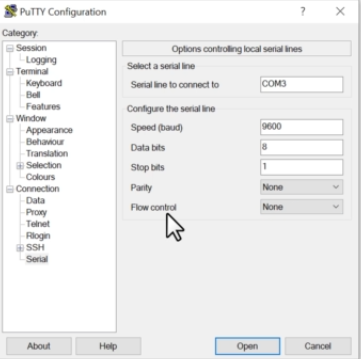
\includegraphics[width=0.4\textwidth]{./Figs/2021-10-14-22-47-00.png}
% 	\caption{}
\end{figure}
Return to the 'Session' tab and click on 'Open'. Now turn on your router, you will start to get output on the screen. The next thing is that the router will boot up, this will take some time so give it some time.

\subsection{Console connection troubleshooting}
\begin{itemize}
    \item When we buy a new device we saw how we can make the initial configurations including adding the IP addresses in order to connect to it over the network.
    \item As well as for initial configuration, the console port - and cable - can be used if the device's IP addresses become unresponsive.
    \item It can also be used to troubleshoot the bootup process. You can view the device booting up from a console connection but this is not possible with SSH because the system must have booted already before the IP addresses will be live.
    \item Another case is when a device just appears to be completely unresponsive but you can see that the device is on, that indicates that the device is probably failing to boot up. Again trying to connect to it over the network will not work, you need to take out your console cable and troubleshoot it. It will not work by connecting to it because the IP is only live until it has completed the bootup process, therefore you cannot connect it through the network, but you can connect to it over the cable and power the device on and you can watch if any problems ensue.
\end{itemize}
